%----------------------------------------------------------------------------------------
%	PACKAGES AND OTHER DOCUMENT CONFIGURATIONS
%----------------------------------------------------------------------------------------

\documentclass{article}
\usepackage{array}
\usepackage[english]{babel}
\usepackage[letterpaper,top=2cm,bottom=2cm,left=3cm,right=3cm,marginparwidth=1.75cm]{geometry}
\usepackage{amsmath}
\usepackage{graphicx}
\usepackage{float}
\usepackage[colorlinks=true, allcolors=blue]{hyperref}
\usepackage{todonotes}
\usepackage{setspace}
\onehalfspacing
\graphicspath{ {resources/} }

\title{Heimdall - A Kubernetes Extension}
\author{Bryan Keane}

\begin{document}

\begin{titlepage}

    \newcommand{\HRule}{\rule{\linewidth}{0.5mm}} 
    \center
    
    
    %----------------------------------------------------------------------------------------
    %	LOGO SECTION
    %----------------------------------------------------------------------------------------
    \begin{center}
        
\includegraphics{setu_logo.png}
    \end{center}
     
    %----------------------------------------------------------------------------------------
    
     
    %----------------------------------------------------------------------------------------
    %	HEADING SECTIONS
    %----------------------------------------------------------------------------------------
    \textsc{\Large Bachelor of Science (Hons) Applied Computing}\\[0.25cm]
    
    
    %----------------------------------------------------------------------------------------
    %	TITLE SECTION
    %----------------------------------------------------------------------------------------
    
    \HRule \\[0.75cm]
    { \huge \bfseries Heimdall - A Kubernetes Extension}\\[0.3cm] %document
    \HRule \\[1.0cm]
     
    %----------------------------------------------------------------------------------------
    %	AUTHOR SECTION
    %----------------------------------------------------------------------------------------
    
    \begin{minipage}{0.4\textwidth}
    \begin{flushleft} \large
    \emph{Author:}\\
    Bryan Keane 
    \end{flushleft}
    \end{minipage}
    ~
    \begin{minipage}{0.4\textwidth}
    \begin{flushright} \large
    \emph{Supervisor:} \\
    Lucy White
    \end{flushright}
    \end{minipage}\\[2cm]
    
\end{titlepage}

\newpage

\tableofcontents
\newpage

\listoffigures
\newpage




\section{Plagiarism Declaration}
I declare that this material, which I now submit for assessment, is entirely my own work and has not been taken from the work of others, save and to the extent that such work has been cited and acknowledged within the text of my work. I understand that plagiarism, collusion, and copying are grave and severe offences in the university and accept the penalties that would be imposed should I engage in plagiarism, collusion or copying. I have read and understood the Assignment Regulations. I have identified and included the source of all other facts, ideas, opinions, and viewpoints in the assignment references. Direct quotations from books, journal articles, internet sources, module text, or any other source are acknowledged and the source cited are identified in the bibliography. This assignment, or any part of it, has not been previously submitted by me or any other person for assessment on this or any other course of study.  



\newpage
\section{Acknowledgements}
I would like to express my deepest appreciation to my Mentors Ciaran Roche and Laura Fitzgerald who provided invaluable experience and contributions to this project. I would also like to extend my deepest gratitude to my Project Supervisor Lucy white for guiding and encouraging me throughout the process.



\newpage
\section{Introduction}
This project, Heimdall, is an open-source Kubernetes Extension built for multi-operator Kubernetes environments. Implementing Heimdall will allow developers to configure it to watch resources of their choosing in a Kubernetes cluster. Heimdall will prevent any unwanted Operators from changing that resource, while simultaneously sending an interactive notification to the developer via a pre-configured Slack Channel regarding the issue. 



\subsection{Background}
In 2022 I completed an 8-month internship at Red Hat for my 3rd-year work placement. I worked on the Red Hat OpenShift API Management (RHOAM) team. RHOAM utilises multiple OpenShift Operators, which are automatically managed and configured applications, to provide a comprehensive API solution to its customers. The API management features provided by RHOAM include: \cite{rhoam-overview}
\begin{itemize}
    \itemsep0em 
    \item Limiting the number of API requests based on the customer’s quota
    \item Creating security policies to manage API access
    \item Monitoring API health
    \item An API portal for sign-up and documentation
\end{itemize}
While working on this team, I had the opportunity to contribute to applications which utilize various technologies like Kubernetes, OpenShift, and Go Operators.



\subsection{Motivation} 
Throughout my internship, I ran into a number of technical issues. One such issue centred around RHOAM's rate-limiting service which has become the motivation for my final year project, Heimdall. The issue in question was with the port through which API requests were being sent in order to be rate limited. That port was being overwritten by a conflicting Operator who had a different desired state for that resource. Rate limiting in this context refers to the maximum number of API calls allowed during a specified time period \cite{understanding-apis} \\\par RHOAM uses the Marin3r Operator to provide rate-limiting for RHOAM customers. It works by injecting a rate-limiting container into a Pod. The container then acts as a middleman for API requests by only redirecting requests to the destination container if the API request limit has not been reached. A more detailed explanation of this process will be discussed in \hyperlink{technologies}{Section \ref{technologies}}. \\\par It took several days of debugging to figure out what was going wrong and another week passed before my fix was merged. This meant that this problem had been occurring on customer clusters before my fix was rolled out to production. After speaking to developers on various Red Hat teams, it became apparent that this problem was not unique to our team and in fact, was an issue that all Kubernetes and OpenShift product teams face. Fixing this will not only benefit Red Hat teams but any team working on a Kubernetes-based application that utilizes Operators.


\newpage
\subsection{Problem Statement} \label{problem-statement}
In Kubernetes (K8s), resources (or objects) have a desired state which describes what the actual state of that resource should look like. The desired state can either lie in a YAML definition or in the code of a Controller. Operators and Controllers can watch that resource's actual state and continuously compare it with the desired state. If they do not match then it is the job of that Operator or Controller to make the necessary changes in order to synchronise them \cite{operator-pattern}.

\begin{figure}[H]
    \hypertarget{problem-model}
    \centering
    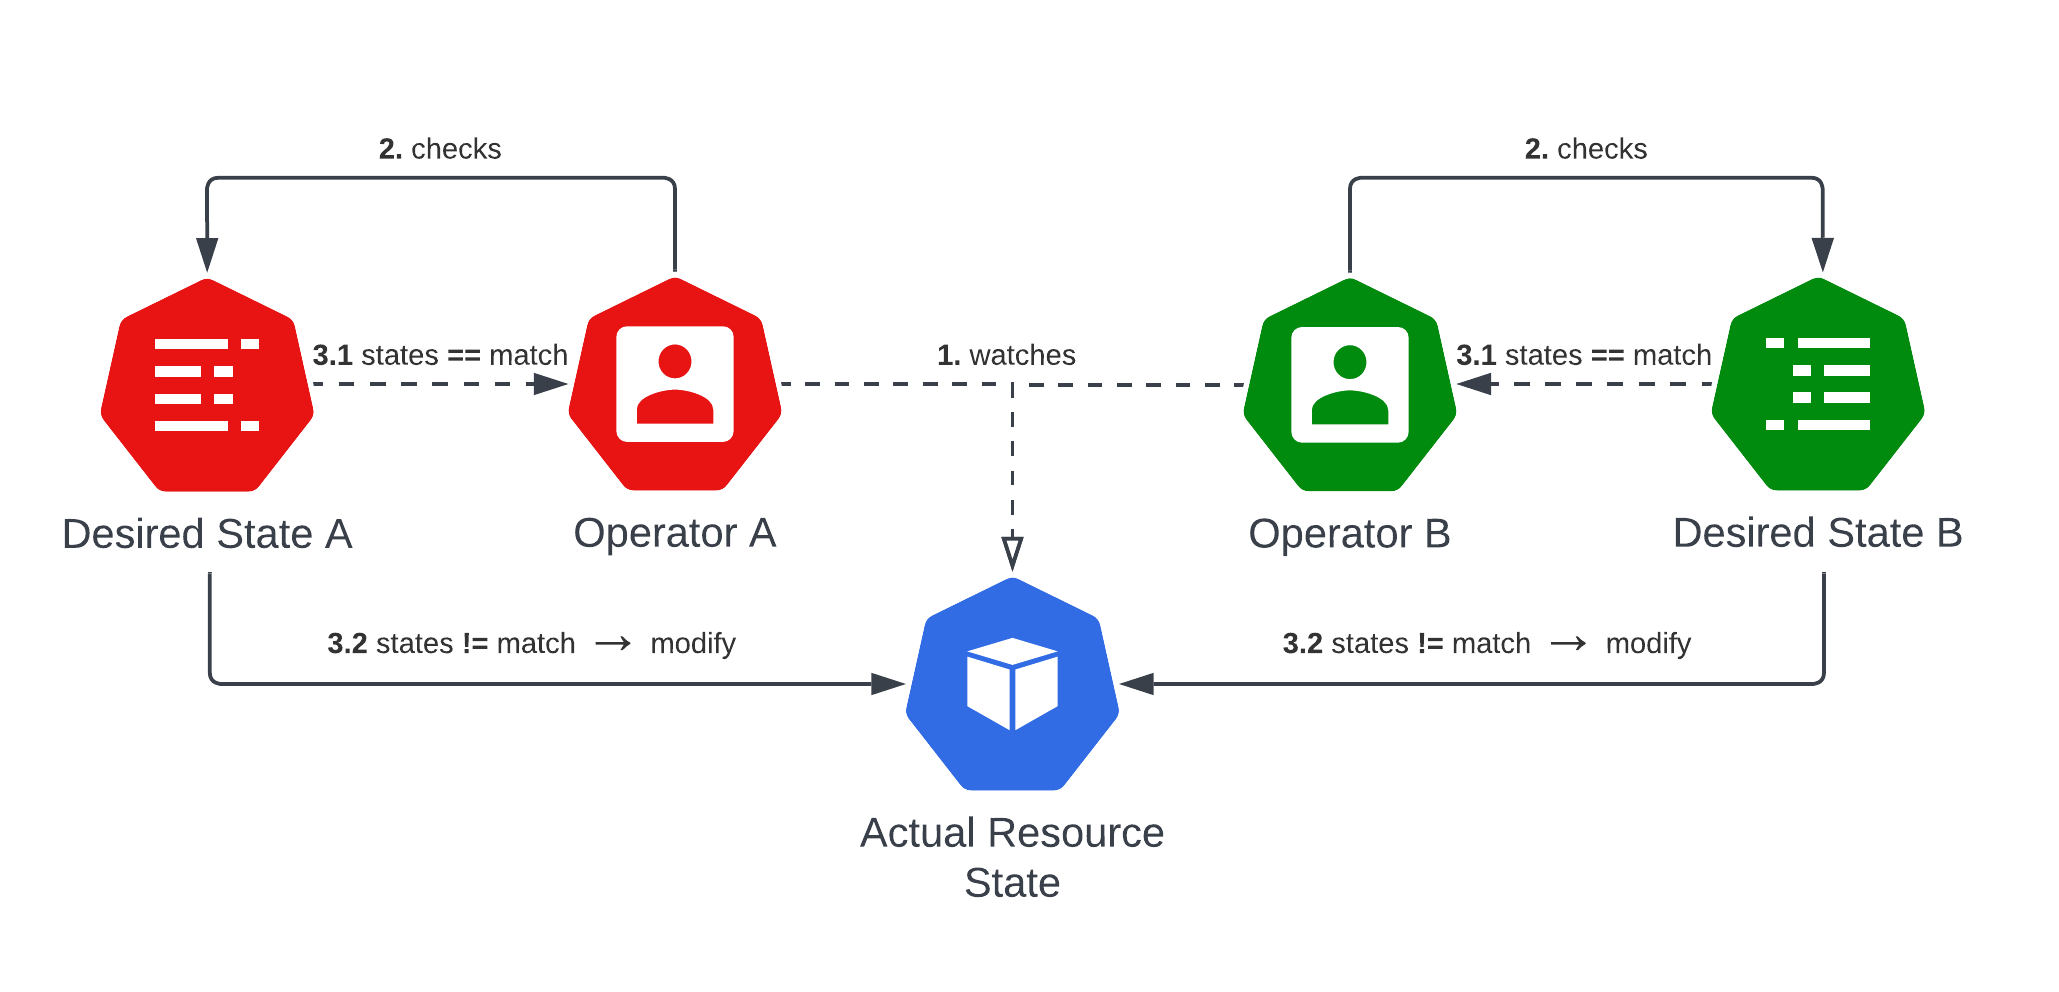
\includegraphics[width=150mm]{intro/problem-model.png}
    \caption{\emph{Model of The Problem - Two Operators Fighting Over a Resource's State}}
    \label{problem-model}
\end{figure}

This pattern works well until two Operators with conflicting desired states are both set to reconcile a resource. This will cause the resource's state to continuously change as both Operators attempt to synchronise its actual state with their unique desired state. The model shown in \hyperlink{problem-model}{Figure \ref{problem-model}} shows this problem in action. Each Operator will do the following:
\begin{enumerate}
    \itemsep0em 
    \item Watch a resource's actual state.
    \item Check the desired state for that resource.
    \item Compare the actual state with the desired state and
    \subitem 3.1. \emph{If they match} then return to Step 1. and repeat.
    \subitem 3.2. \emph{If they don't match} then modify the resource's actual state.
    \item Repeat this process continuously.
\end{enumerate}



\subsubsection{Industry Example}
As an example, the open-source e-learning platform Moodle can be used. In an educational environment, one might have a Moodle Operator and a MySQL Operator to serve as Moodle's database. The MySQL Operator manages the storing, of course, student, and module information. This application may then install a Tutors Operator, which is another e-learning platform which houses course notes and lab work. Since there is already a MySQL database via the MySQL Operator, Tutors can use the same database to store course notes and lab work. 

\begin{figure}[H]
    \hypertarget{moodle-tutors}
    \centering
    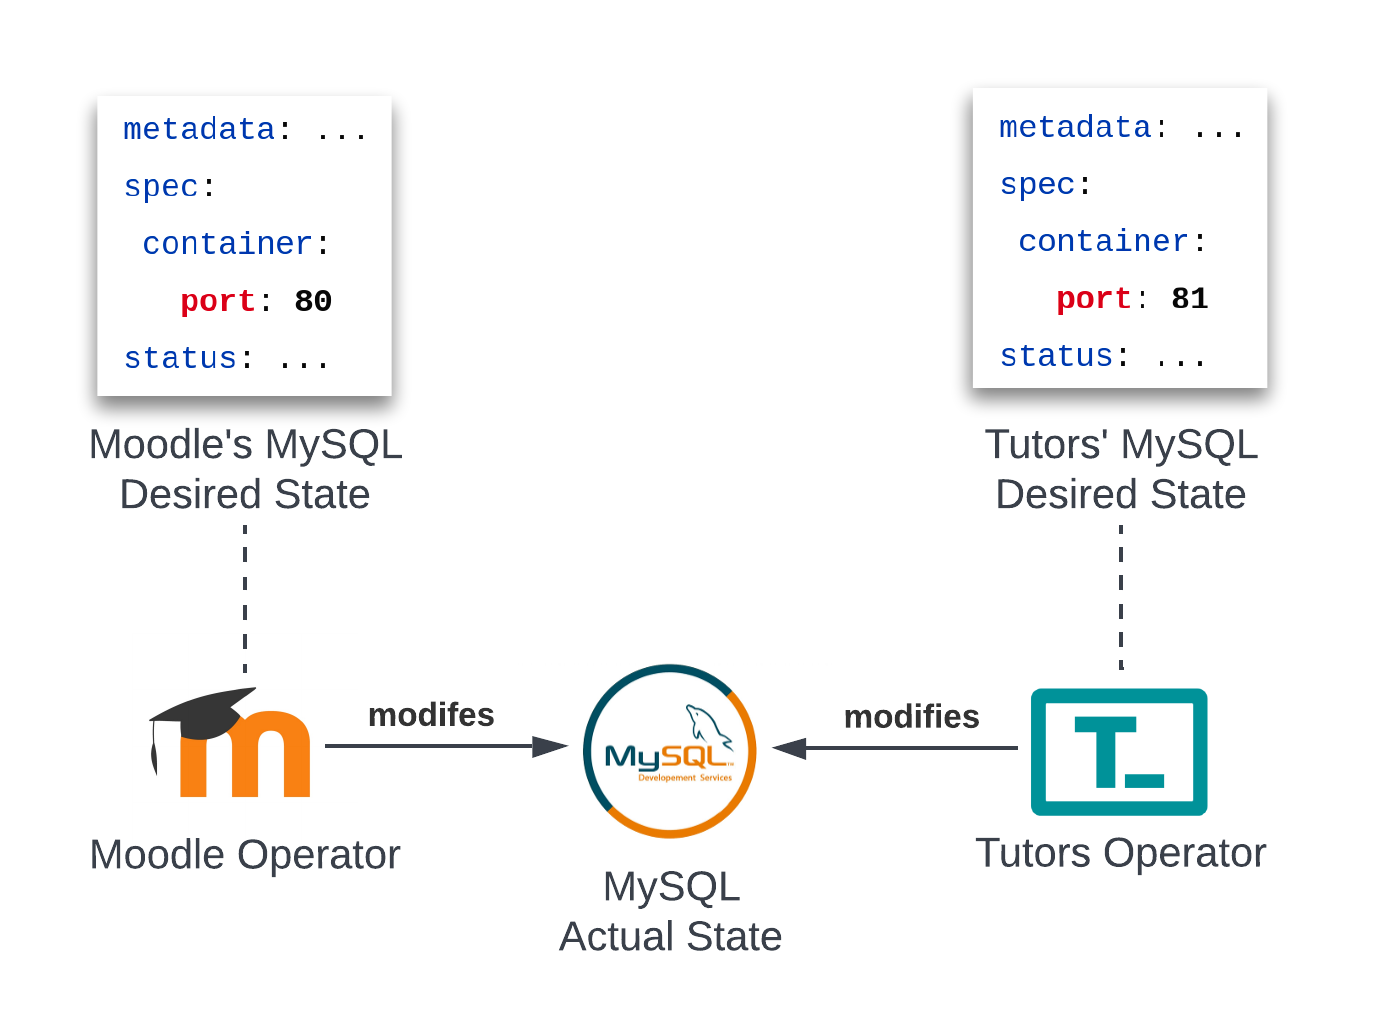
\includegraphics[width=125mm]{new-moodle-example.png}
    \caption{\emph{Simplified Model of Moodle, Tutors, and MySQL Industry Example}}
    \label{moodle-tutors}
\end{figure}

In this example, it would be very easy to misconfigure one of the Operators to have a dissimilar desired state for the MySQL resource. This would cause both Operators to constantly change that resource. Imagine Moodle wanted the port in which database access occurred to be port 80 and Tutors wanted the database access to occur through port 81. This would cause the MySQL resource's access port to be changed back and forth. If a lecturer or student attempts to access information through Moodle, but at that point in time the MySQL resource's port was configured by the Tutors Operator, the user would not be able to retrieve the data. 

\subsection{Aims and Objectives}
The solution is to create a custom Kubernetes controller which will monitor resource states. A Kubernetes Operator can create a resource, become its owner, and will set the controller to watch that resource for changes. If another operator changes the resource the controller will trigger an alert, notify the developer via a slack integration and allow the developer to fix the problem without the need for time-consuming debugging. 

\begin{figure}[H]
    \hypertarget{solution-model}
    \centering
    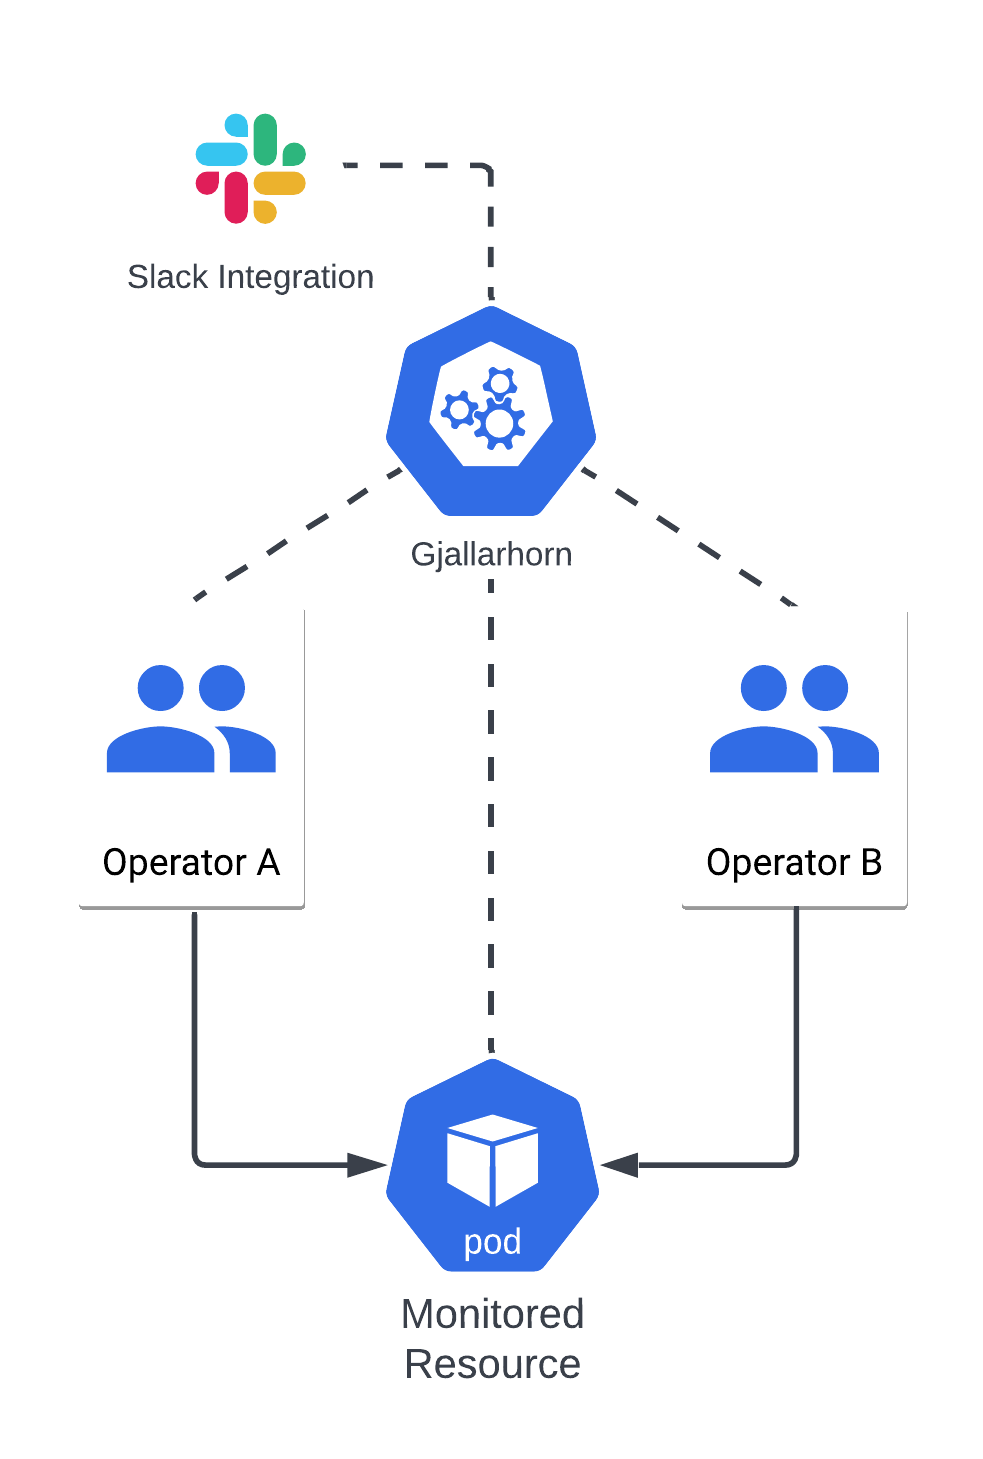
\includegraphics[width=100mm]{solution-model.png}
    \caption{\emph{Model of the solution: Heimdall}}
    \label{solution-model}
\end{figure}

\hyperlink{solution-model}{Figure \ref{solution-model}} models the proposed solution where the Owner Operator and Rogue Operator are attempting to change a resource's actual state. Once the Owner Operator is installed, it creates the resource with the addition of a label that Heimdall is looking for. Heimdall sees a new resource created with this label and begins monitoring its state. The Rogue Operator is installed and begins changing the resource. \\\par The minimum viable product for Heimdall involves the controller watching for non-owners changing the state of a resource. It will then generate an interactive notification for slack with details on the issue to allow the developers to find and fix the problem with relative ease. The stretch goals for Heimdall will achieve the following:
\begin{enumerate}
    \itemsep0em 
    \item Allow for an atomic owner of a resource to be set.
    \item Block changes to resources from non-owners.
\end{enumerate}

This will not only allow the developer to fix the problem with ease but also stop the issue from occurring and prevent any downtime for the end user. These will be discussed further in Section \ref{stretch-g}. 


\newpage

\section{Design}

This section will begin by outlining the functional and non-functional requirements that the controller must fulfil in order to be effective, including the ability to install on any Kubernetes environment, connect to Slack for notifications, block changes to resources from unwanted operators, and provide supporting documentation. Next, an overview of the architecture of Heimdall will be presented to give a deeper understanding of how the technical components of the Controller will operate. Lastly, each aspect of the project will be discussed in depth in order to fully understand the project and its components.


\subsection{Requirements} \label{requirements}

There are various requirements for the successful implementation of Heimdall. These requirements can be divided into two categories: functional requirements and non-functional requirements. Functional requirements describe the specific capabilities or features that the system must have, while non-functional requirements describe constraints that the system must adhere to \cite{func-vs-nonfunc}. It is important to carefully define both types in order to ensure that Heimdall meets the needs of its users and operates in a reliable manner. These will serve as a guide for the design and development of the Controller and will help to ensure that it is able to effectively detect and resolve conflicting Resource changes between Operators in a Kubernetes cluster.


\subsubsection{Functional Requirements}

Functional requirements are features and capabilities that the system must possess in order to meet the needs and expectations of the user. In the case of Heimdall, these requirements are primarily focused on the functionality that will be most useful to developers implementing the controller into their environments, as well as site reliability engineers installing it onto customer Kubernetes clusters. Heimdall's Functional Requirements are as follows:

\begin{enumerate}
    \itemsep0em
    \item Developers must be able to install the controller on any Kubernetes cluster.
    \item Developers must be able to configure the controller to connect to Slack for notifications.
    \item Developers must be able to define an Operator that is unable to make changes to the specified Resource.
    \item Developers must have access to appropriate documentation which outlines the proper configuration and use of Heimdall.
\end{enumerate}

With the functional requirements outlined, the following section will delve into the technical details necessary for the successful implementation of these end-user features.

\subsubsection{Non-Functional Requirements}

Non-Functional Requirements are technical specifications that help ensure that the system meets the desired functional requirements. They define the performance, reliability, security, and other characteristics that the system must possess in order to function effectively. Heimdall's Non-Functional Requirements are as follows:
\begin{enumerate}
    \itemsep0em
    \item Heimdall must be able to use the Unstructured Package to watch Resources of any type, including Core and Custom Resources.
    \item When a Resource is watched, events on it should trigger a Reconcile for that Resource.
    \item During a Reconcile, Heimdall must verify if events are coming from the owner Operator or not.
    \item If the event is coming from a non-owner, Heimdall must configure a new Role and Role Binding to grant the correct permissions to that Operator's Service Account.
    \item The Controller must also handle the reconciliation of the Slack integration, including:
    \subitem a. A Config Map storing the Slack channel information that Heimdall sends notifications to.
    \subitem b. A Secret storing the Slack API Key that Heimdall uses to send Slack messages.
    \item Heimdall must use the Slack Go Client to send messages to a Slack Channel with information from the Config Map and Secret.
    \item These messages must be interactive and provide a link to the affected Resource.
    \item Finally, Heimdall must have a working and publicly available Docker image built for installation.
\end{enumerate}

These requirements provide the foundation for the design of the system, as they outline the necessary capabilities and technical considerations that must be taken into account. In the following section, we will delve deeper into the architecture of Heimdall and discuss how these requirements will be implemented and integrated into the overall design of the system.

\subsection{Architecture Model}

The design of Heimdall is illustrated in Figure \ref{arch-diag}, which shows how the controller will function when the minimum viable product and stretch goals are implemented. This figure includes the responsibilities of the Controller in the context of an example scenario and details the various moving parts involved in the implementation. In the following section, we will delve deeper into the specific components and processes of Heimdall, providing a more detailed understanding of how the controller functions and achieves its functional and non-functional requirements.

\begin{figure}[H]
    \centering
    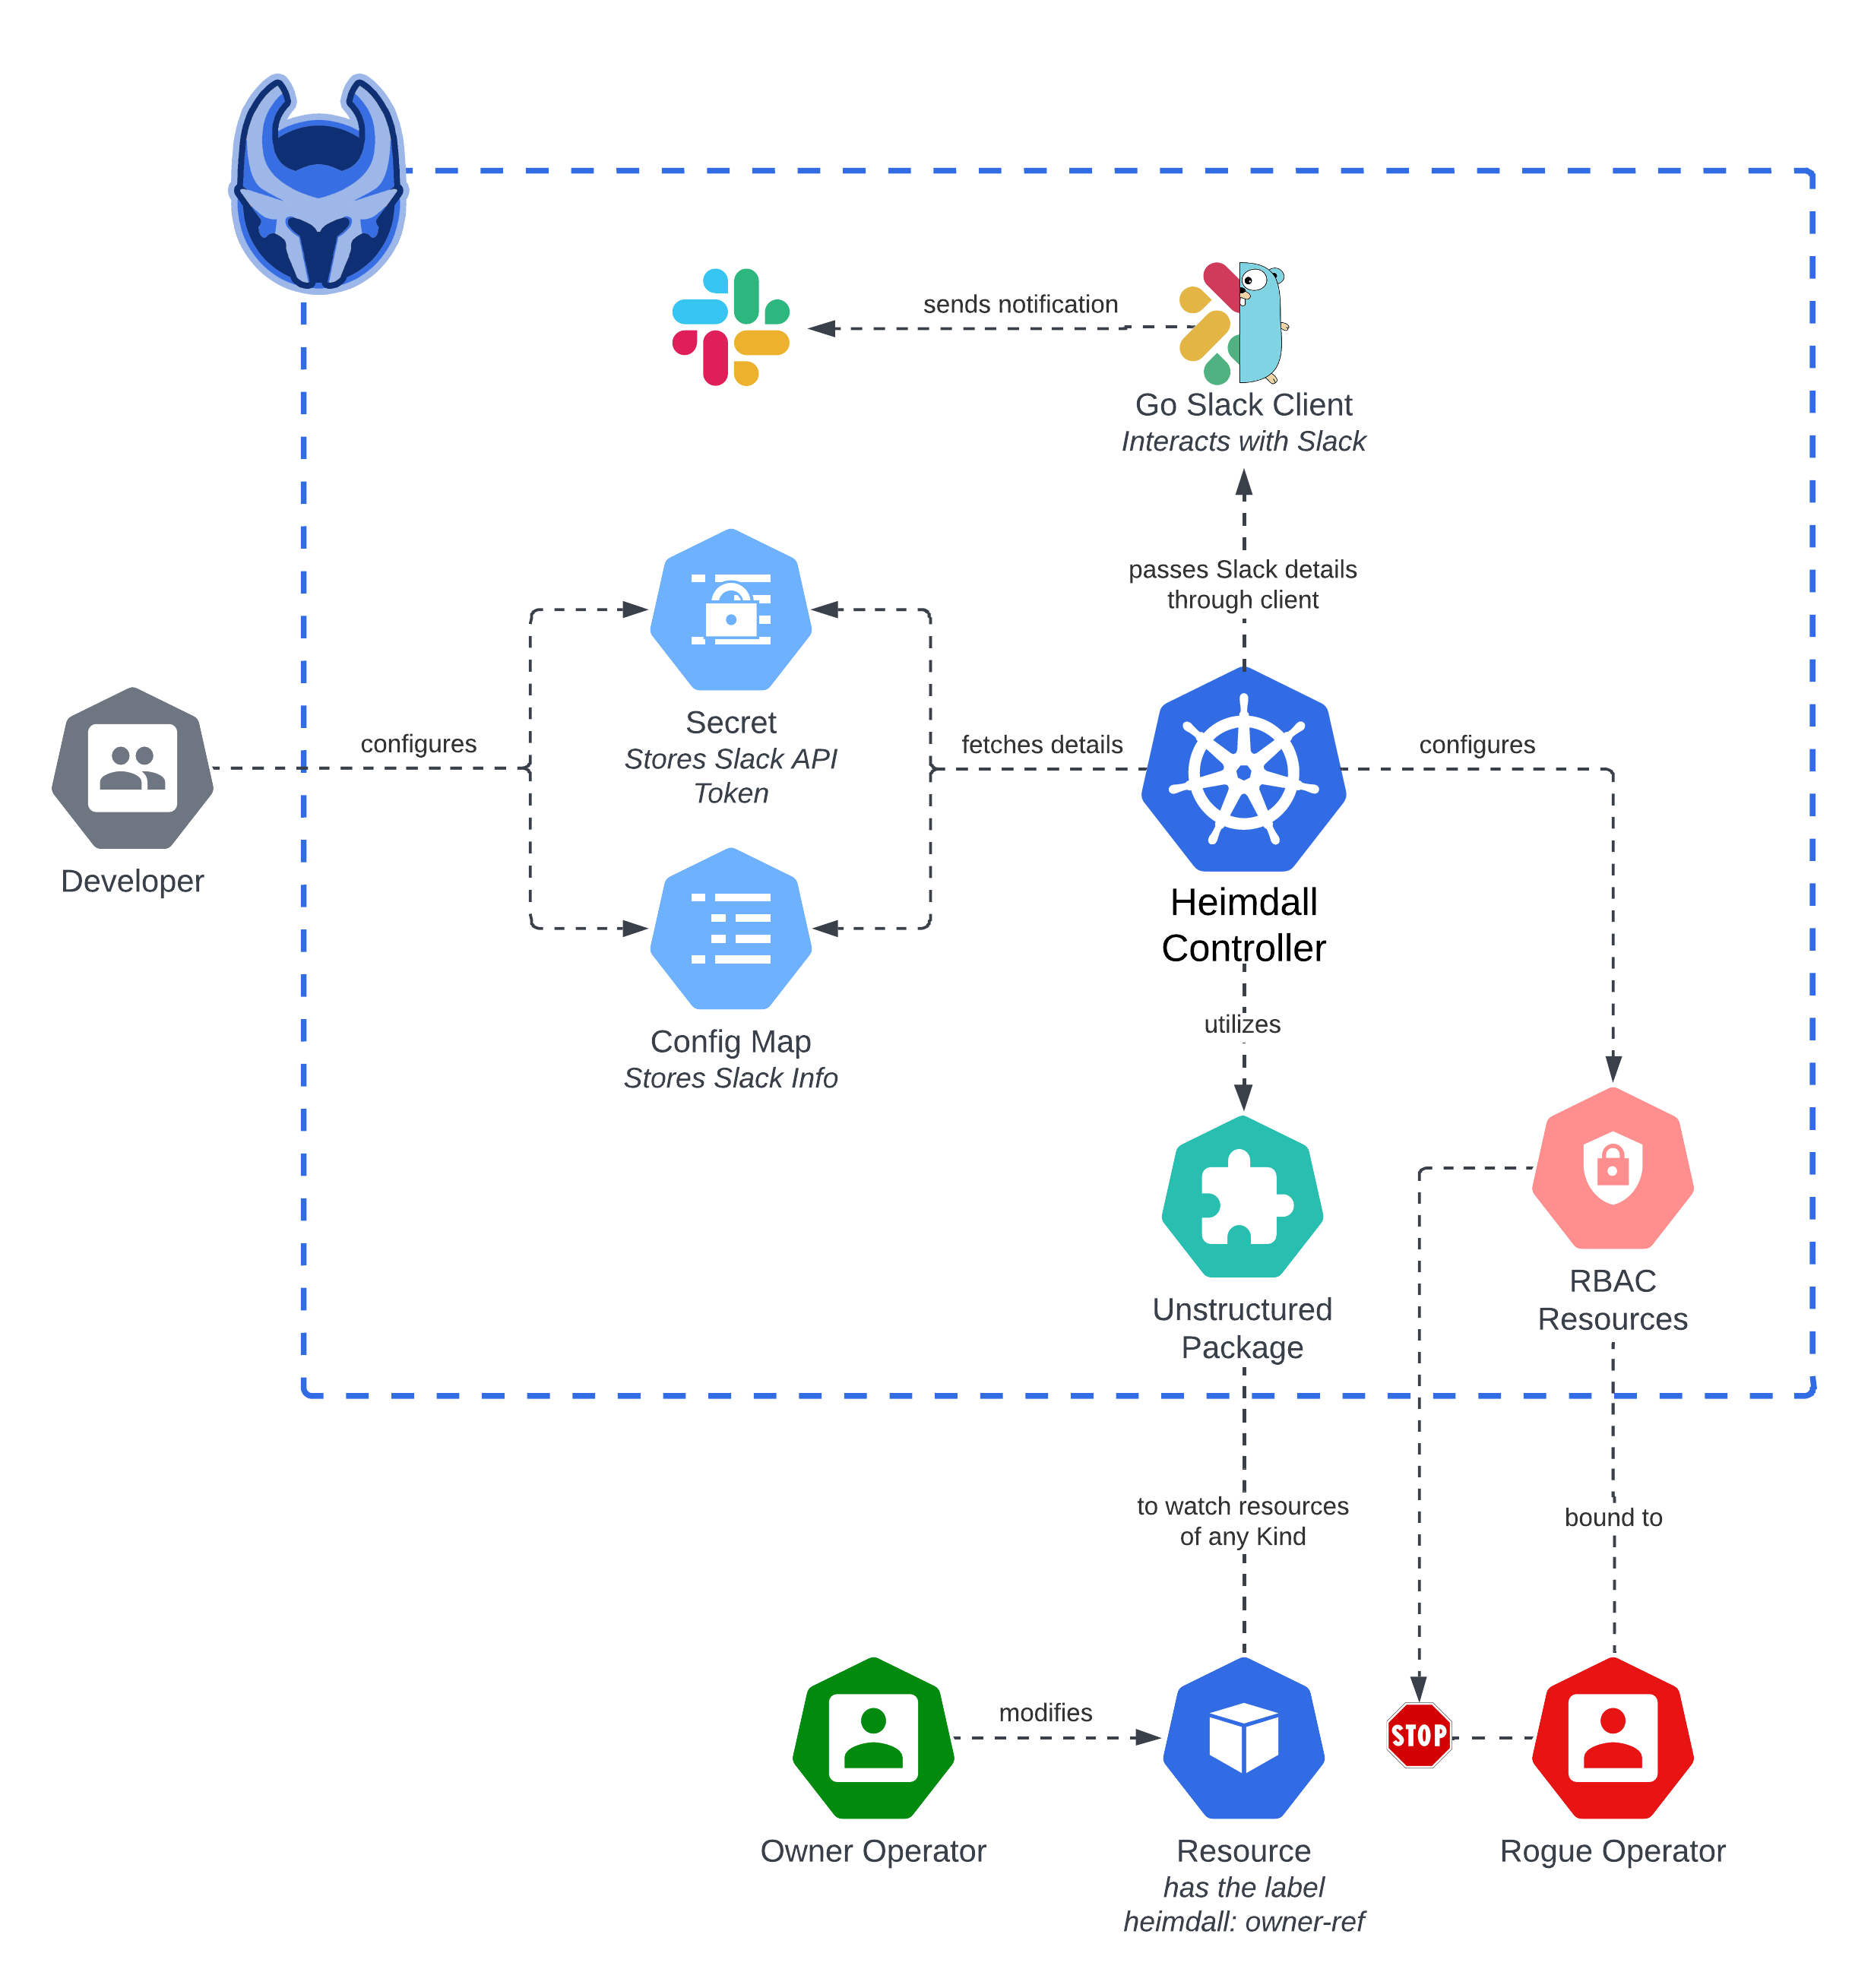
\includegraphics[width=160mm]{design/arch-diag.png}
    \caption{\emph{Heimdall system architecture overview model}}
    \label{arch-diag}
\end{figure}


\subsection{System Design} \label{design-desc}

The system design aims to provide a detailed description of the various components involved in the implementation of Heimdall. This section will cover the Controller Overview, the use of the Unstructured Package, Slack Integration, Role Based Access Control, and Installation. 

\subsubsection{Controller Overview}

The Controller is the centre-piece of Heimdall. It is what makes this entire project work and will house the majority of the code. As most Kubernetes Controllers do, Heimdall's Controller will have two main functions at the very least. The first of which is the \emph{Add} function. This will initialize the Controller itself using the \emph{controller-runtime} package, which is discussed in Section \ref{osdk}, and will utilize the Unstructured Package to set a Watch on specific Resources. Once a Watch is set on a Resource, this triggers the second main function \emph{Reconcile}. This function will house a lot of the logic carried out by Heimdall. When an event occurs on a Watched Resources, the Reconcile function will carry out the logic to identify whether the change came from the owner or a rogue Operator. If the event came from a rogue Operator, it will then trigger two main pieces of code: the Slack Notification and the reconfiguration of Role Based Access Control Resources to block any future changes to that Resource from that Operator.

\subsubsection{Unstructured Package Implementation}

As part of the Heimdall Controller, the Unstructured package must be used in order to Watch Resources of any type in a Kubernetes cluster. This package provides a means by which to convert any type of Object in a Kubernetes cluster and turn it into a generic type. This will allow Heimdall to not have to declare the resource type when setting a Watch on Resources, so it can essentially Watch any resource in a cluster. This is especially helpful for Custom Resources as Heimdall needs to be installed and configured to work with any Kubernetes environment, so it needs to be dynamic in the way that it deals with Resources of different types.

\subsubsection{Slack Integration}

The integration with Slack involves a few different steps. The main components are the Config Map, the Secret, and the Slack Go client. Heimdall will first need to Reconcile the Config Map and the Secret. If either of them does not already exist in the cluster, the Controller will create them. This is so both Resources are guaranteed to be present on the cluster and ready for the Developer to configure them. Once they are configured correctly with the Slack API Token and the Slack Channel name, Heimdall can use that information to send Slack messages. The messages sent will need to be somewhat interactive. Ideally, this would include a link to the affected Resource, but at the very least it should contain the Name and Namespace of the Resource, the event type, and the source of the unwanted changes.

\subsubsection{Role Based Access Control} \label{security}

Upon a watched Resource being changed by a non-owner, Heimdall will detect that change and trigger the Reconcile function for that Resource. To stop any new changes from being made by that Operator, the Controller must create new RBAC Resources like Roles and Role Bindings. The Roles will be bound to the Operator's Service Account with new Role Bindings so that when that Operator attempts to make another change to the watched Resource, it won't have the correct permissions. This functionality is subject to change as it has not yet been attempted and is not confirmed to be possible in a production environment. Upon actually implementing this functionality, it may differ slightly from this design.


\subsubsection{Installation}

Lastly, Heimdall needs to be installable via a public Docker image. An image can be built and pushed to a public container image repository like Docker Hub or Quay. This image can then be used by any developer that needs to implement Heimdall into their environment and run on the cluster. Appropriate documentation will need to exist so that the installation and configuration are easy to complete. This documentation should also include steps to create a Slack API for the developer's Slack Channel, and how to configure the Config Map and Secret correctly.



\subsection{User Stories}

User stories are a way of expressing requirements for a product in a way that is easily understood by a product's stakeholders. They are used in Agile development, as discussed in Section \ref{agile}, and are an important tool for creating a shared understanding of the desired functionality of a product \cite{user-stories}. User stories help to focus on the value that a feature will provide to the end user and provide a framework for refining its requirements. The following are Heimdall's user stories:

\begin{itemize}
    \itemsep0em
    \item As a Developer, I want to be aware of changes to resources that I own so that I can take action if an unwanted change is made.
    \item As a Developer, I want to control the cadence of alerts so that I can control the noise created by those alerts.
    \item As a Developer, I want to claim ownership of the resources that I control.
    \item As a Developer, I want to control the changes to resources that I own.
\end{itemize}

These provide clear and concise descriptions of the desired functionality of Heimdall and will serve as a guide for the development team next semester.

\subsection{Risk Analysis}

There are a number of risks associated with this project's implementation, one of which is far more significant than the others. During the initial research into the viability of this project, there were no examples or previous attempts found that try to implement such a solution. This poses a significant risk as it means that it is not guaranteed that the implementation will be technically possible. An appropriate risk mitigation strategy is needed in order to ensure that the creation of Heimdall can still be completed to some degree. To do this, the project has been split up into a Minimum Viable Product (MVP) and stretch goals which are discussed further in Sections \ref{mvp} and \ref{stretch-g}. If after exhausting all attempts to implement the stretch goals, it is found that it is not possible, the MVP still provides a valid solution to the problem. \\\par If the implementation is confirmed to be technically possible, the next risk will be that the project cannot be completed within the given time constraint. Again, this can be partially mitigated by the use of the MVP and stretch goals. Although, with the use of the chosen methodologies discussed in Section \ref{methodology}, the use of Sprints and following a Continuous Delivery approach to development should mitigate any concerns about time.



 
\section{Methodology} \label{methodology}

This section will outline the Agile methodology that has been adopted for the development of Heimdall, as well as the version control, continuous integration, and continuous delivery practices that will be implemented to ensure the smooth development of the project. Additionally, we will delve into the testing approach taken and the decision to open-source the project.


\subsection{Agile and Scrum} \label{agile}

Agile is a project management and development method that helps teams deliver value to customers more efficiently. It is based on the idea of continuously iterating on and improving a product through the collaboration of various teams \cite{what-is-agile}. Agile has been chosen because it allows for a more iterative and flexible approach to development. By focusing on delivering the most important features first, there is a higher probability of being able to successfully implement the minimum viable product as well as the stretch goals. \\\par Scrum on the other hand is a framework for Agile development that emphasizes collaboration, flexibility, and the ability to respond to change. One way that Agile teams track progress is through the use of Scrum artifacts such as burndown charts. While the Scrum roles of Scrum Master, Product Owner, and Development Team may not be applicable to a one-developer project like Heimdall, the use of these artifacts will still be useful in monitoring progress and ensuring that the project stays on track.


\subsection{Scrum Artifacts} \label{artifacts}
Teams who practice Agile and Scrum methodologies often collect Scrum Artifacts. These are pieces of information that a product's stakeholders and the team developing it use to describe its development. The main Scrum Artifacts used for this project include Product Backlog Refinement, Sprint Planning, and Sprint Reviews. There are also various Extended Artifacts that are not included in the official Scrum Artifacts definition. These include reporting mechanisms like Burn down Charts.



\subsection{Version Control} \label{version-ctrl}
What is VCS, Git, GitHub 



\subsection{Continuous Integration} \label{ci}
Version control lies at the heart of Continuous Integration. CI is an Agile practice of integrating code changes to a product automatically from various contributors (product teams and open-source community contributions). It is a method used to consistently merge code changes into one central repository which runs automated tests and builds to ensure code functionality and integrity.   


 
\subsection{Continuous Delivery} \label{cd}
Continuous Delivery is an approach 



\subsection{Testing Approach}



\subsection{Open Source} \label{open-source}



\section{Technologies} \label{technologies} 



\subsection{Kubernetes}

Kubernetes is an open-source tool used to implement modern micro-service-based architectures. It can be used to create, manage, and deploy containerized applications and is commonly known as a container orchestrator \cite{k8s-overview}. Containers are small processing units which house applications and their dependencies. They are bundled up into a singular image that is able to run on any hardware. This removes the need for installing required packages when attempting to run an application. Kubernetes orchestrates the deployment of many containers to form larger applications that are highly available, fault-tolerant, and have high degrees of redundancy.



\subsubsection{Resources} \label{resources}

Resources, also known as objects, are how the state of a Kubernetes cluster is represented. These resources are detailed in \emph{.yaml} format \cite{k8s-obj}. They usually describe the following key pieces of information:

\begin{itemize}
    \itemsep0em 
    \item Which container image is being used
    \item The compute resource available to the application, namely CPU and Memory limits
    \item Resource policies on how things like fault tolerance, upgrade behaviour, and restart behaviour should operate
    \item General resource information like the Namespace, Labels, and Annotations
\end{itemize}

The lowest-level Kubernetes resource is a Pod. Pods house the containers that run applications. They are expendable and can never be edited. If the desired state of a Pod is changed, it is destroyed and recreated to match the Pod's actual state with the new desired state. This also increases the cluster's degree of fault tolerance as if one Pod fails, instead of trying to recover it the Pod can be deleted and redeployed. 

\begin{figure}[H]
    \centering
    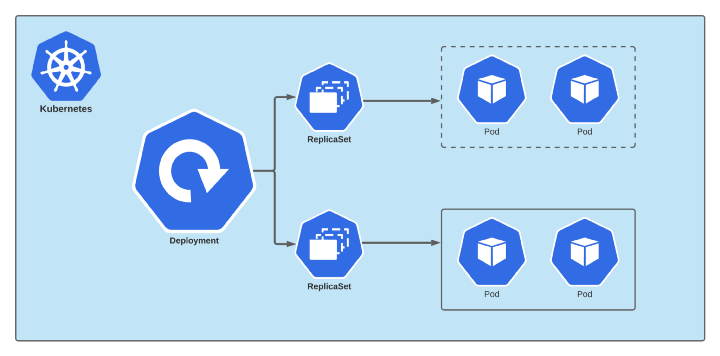
\includegraphics[width=160mm]{tech/resource-struct.png}
    \caption{\emph{Kubernetes application Resources: Deployments, Replica Sets, and Pods}}
    \label{resource-struct}
\end{figure}

There are two other Resources which make up the structure of a running application in Kubernetes. Figure \ref{resource-struct} \cite{k8s-rolling} details how Deployments and Replica Sets work with Pods in order to complete an application's workflow. Deployments are the top-level Resources in this structure and typically act as the source of truth (desired state) for Pods. If a Deployment's \emph{.yaml} specification is changed by another Controller, then its Pod's desired state will change and be redeployed. The Deployment also acts as a desired state for Replica Sets, which are responsible mainly for managing the number of Pod replicas currently running. 

\begin{figure}[H]
    \centering
    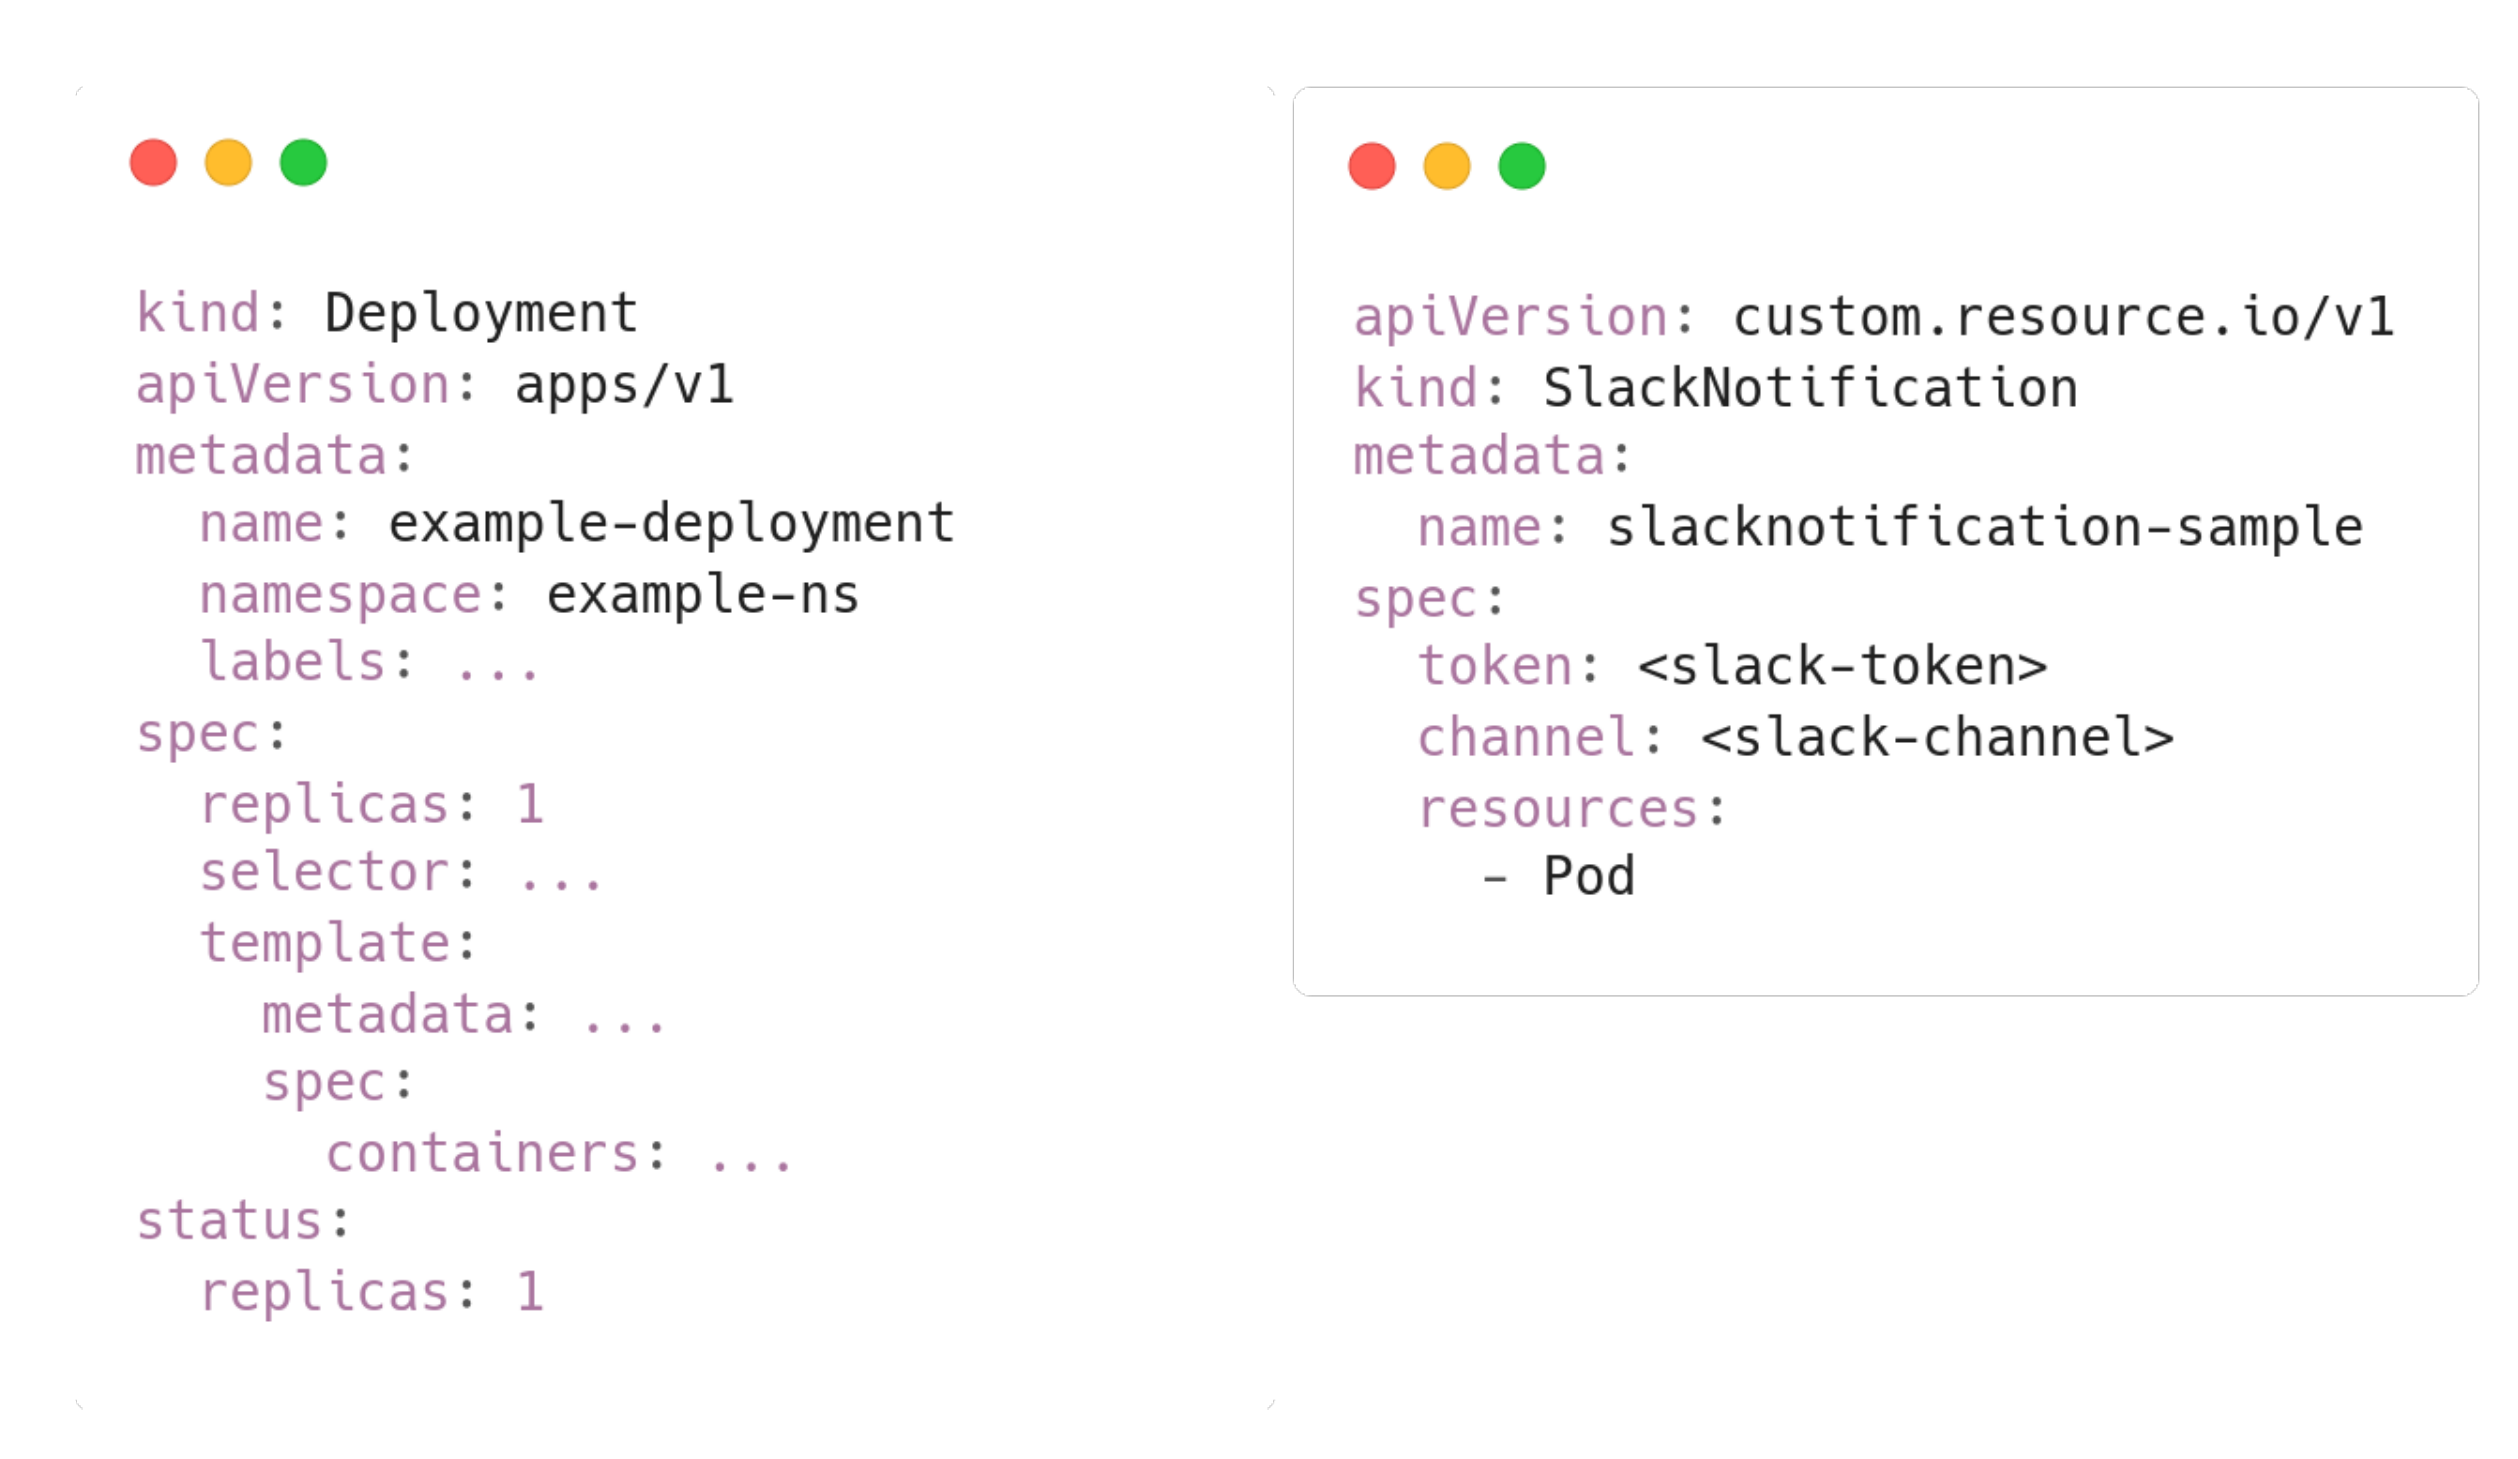
\includegraphics[width=125mm]{tech/core-cr.png}
    \caption{\emph{Example Core Resource (Deployment) comparison with Example Custom Resource}}
    \label{core-cr}
\end{figure}

Additionally, there are Custom Resources. They extend the Kubernetes API outside of the typically available resource types. They allow for customisation of the typical resource fields like \emph{.spec} and can be reconciled (watched and maintained) by custom controllers \cite{cust-res}. An example \emph{yaml} definition of a Deployment (Core Resource) and a Custom Resource (Slack Custom Resource Example) can be seen in Figure \ref{core-cr}. As seen, the Custom Resource (on the right) can have any custom fields in the Resource's \emph{.spec} and the Kind and API Version values are different to that of Core Resources.



\subsubsection{Controllers} \label{controllers}

As already explored in Section \ref{problem-statement}, Controllers are predominately responsible for watching the actual state of resources and matching it with their desired state. An example would be the Deployment Controller which ships natively on Kubernetes clusters. It ensures that the actual state of all Pods matches their desired state described in its Deployment. Custom Controllers can also perform various different operations including interacting with services outside of a cluster, like sending notifications to a Slack Channel \cite{ctrlrs-ref}. Custom Controllers and Custom Resources packaged up together to create one application are what Kubernetes refer to as the Operator pattern.


\subsubsection{Operators}

The core purpose of Operators is to attempt to perform the actions a human operator might. This includes monitoring, managing, and maintaining an application. This is done instead through code where an Operator is installed onto a cluster and will automatically handle any failures, react to changes in the cluster, and carry out actions upon specific events occurring \cite{operator-pattern}. This could be as simple as managing a web server and scaling up the number of web server pods as it gets more traffic to prevent Pod failure.
\begin{figure}[H]
    \centering
    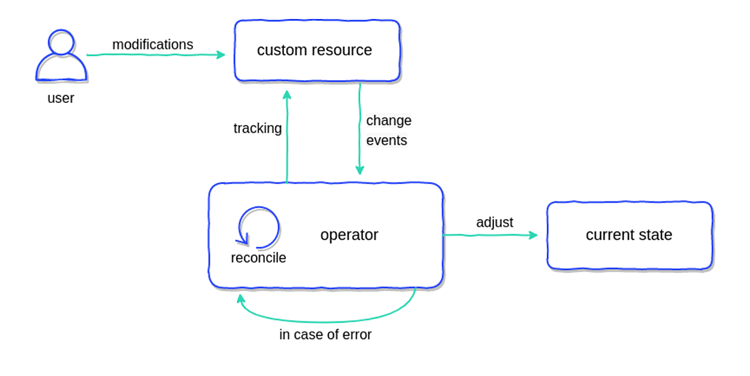
\includegraphics[width=160mm]{tech/operator-pattern.png}
    \caption{\emph{Operator Pattern model of Custom Controller and Resources interaction}}
    \label{op-pat}
\end{figure}

Whatever the use case, they serve the purpose of automating tasks beyond what Kubernetes provides out of the box. A model of the Operator pattern taken from the Container Solutions blog can be seen in Figure \ref{op-pat} \cite{op-pat-blog}. In order for Operators to carry out their intended functions, they need to be granted the necessary permissions.



\subsubsection{Role-Based Access Control}

Kubernetes environments use a Role-Based Access Control (RBAC) method to allow applications to perform certain tasks. Since the API Server acts as a mediator for all Kubernetes actions, the rules which describe a user's permissions use the verbs common to APIs like \emph{GET}, \emph{POST}, and \emph{DELETE} \cite{rbac}. First, applications (Controllers, Pods, Operators, etc) are assigned a Service Account. Roles can then be created which describes what actions any application assigned with that Role can take. Finally, Bindings can be created to link these Roles to specific Service Accounts. This method of permission granting will likely prove useful for the implementation of the Stretch Goal discussed in Section \ref{stretch-g}. These resources are discussed in context in Section \ref{security}.



\subsection{Languages}
There will be two main languages used in the creation of Heimdall, Go and YAML. They are the most commonly used languages when developing Kubernetes applications. This means that supporting documentation is plentiful, and experience with these languages is invaluable.  

\subsubsection{Go}

The Go Programming Language is an open-source language created by Google. It is predominately used to develop cloud and network services, command-line interfaces, web applications, and Developer Operations style projects \cite{go-dev}. Kubernetes Controllers fall under the latter category and since I already have an elementary proficiency with Go, this is the chosen language for Heimdall. The completion of this project will aid in increasing my knowledge and experience with Go, which will be beneficial for my future career.

\subsubsection{YAML}

YAML is a language highly similar to JSON. It is used frequently for defining configurations and is syntactically easy to use \cite{yaml-blog}. Similarly to Go, I have encountered and written YAML at Red Hat, and will be looking to further develop my skills with it during the creation of Heimdall. YAML is the language which defines the desired and actual state of Resources in Kubernetes as discussed in Section \ref{resources}. 

\subsection{Libraries}

Various libraries will be used for the development of Heimdall. Many of these are packaged up in the Software Development Kit discussed in Section \ref{osdk}. 


\subsubsection{Slack Go Client}

The Slack Client for Go (slack-go) allows interaction with Slack channels via code. This client will allow Heimdall to make a connection to a Slack Channel, and send custom notifications containing key information about the problem occurring. This client will be used in the Slack Prototype discussed in Section \ref{slack-poc}.

\subsubsection{Unstructured Package}

Section \ref{controllers} detailed how Controllers can watch specific resources for events. Controllers can be configured to watch Resources which contain a specific label like \emph{heimdall: watching}. This is useful as it means a Controller can watch and perform actions on any Resource which can be dynamically configured. An issue arises when we consider the Resource kind the Controller is being told to watch. If a Controller is set to watch a specific Resource, it requires a Kind to be specified, which could be \emph{Pod}, \emph{Deployment}, etc. What if the Controller is configured to only watch Pods with a specific label but then that label is added to a custom resource which does not contain the kind \emph{Pod}. This is where the Unstructured Package comes into play. This package allows for a Controller to watch and interact with Resources of any Kind. This will be integral to the implementation of Heimdall as the Controller will need to complete its task on any Resource in a cluster regardless of its Kind. This is discussed further in the final proof of concept in Section \ref{unstructured-poc}.



\section{Tools}

The following section will provide an overview of the various tools that will be used throughout the development of Heimdall. These tools are essential for the development of the Controller, the report, and the prototypes. From online LaTeX editors to command line tools for interacting with Kubernetes clusters, these tools will be integral to the success of the project. The section will also provide a brief overview of the purpose and use of each tool, as well as any relevant background information.


\subsection{Overleaf}

Overleaf is an online LaTeX editor and is the tool used to create this report. It will also be the tool used to create the Semester Two report. LaTeX allows the creation of professionally formatted documents using plain text instead of formatted text as typically done with other document writing tools like Google Docs and Microsoft Word \cite{overleaf}.


\subsection{Operator SDK} \label{osdk}

Operator SDK is a Software Development Kit created for building Kubernetes Operators. It provides the necessary tools for the creation of custom Controllers and Resources (custom APIs) and generates a plethora of scaffolding code to get started on an Operator project \cite{osdk-overview}. During this scaffolding process, as seen in Figure \ref{osdk-img}, it can be specified whether or not to generate a Controller and Custom API. In the case of Heimdall, a Custom Resource is not needed so the flag to generate one is left to false.

\begin{figure}[H]
    \centering
    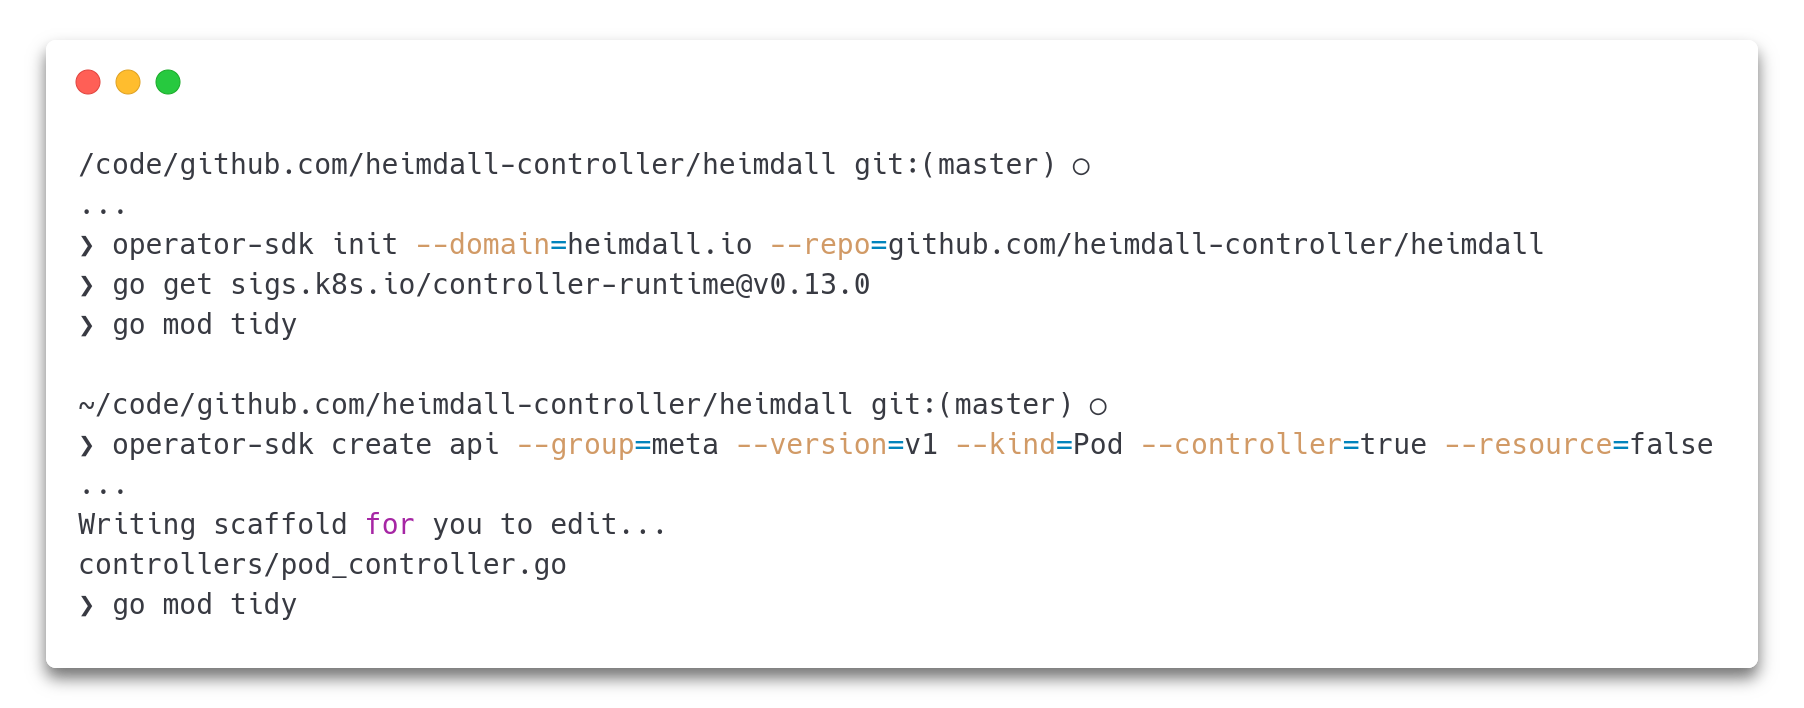
\includegraphics[width=160mm]{tools/osdk.png}
    \caption{\emph{Operator SDK Controller scaffolding via Command Line}}
    \label{osdk-img}
\end{figure}

Aside from code generation, Operator SDK also initialises the use of essential libraries like \emph{controller-runtime} and \emph{controller-tools}. These are sets of libraries that aid in the creation of custom Controllers and will be used extensively during the development of Heimdall.


\subsection{Minikube}

Minikube is a small open-source Kubernetes environment that uses one node (a virtual machine that Kubernetes runs on). It can be run locally and is typically used for the development of Kubernetes applications \cite{minikube-docs}. Minikube provides a dashboard which allows the use of a graphical user interface to configure the Kubernetes cluster and interact with resources. This will be the environment in which Heimdall will be tested. 

 
\subsection{Docker}

Docker is an open-source tool for developing, deploying and shipping containerized applications. Kubernetes uses Docker as its container runtime tool (to run containers) so it plays a large part in a Kubernetes environment \cite{docker-overview}. For Heimdall, it will be used to build and push  custom images of Heimdall so that they can be deployed to any Kubernetes environment. This process of pushing images will also be integral to the release process of Heimdall as discussed in Section \ref{ci}. An alternative to Docker for this purpose is Podman. Podman is another open-source tool created by Red Hat for the same purpose. I have had previous experience with both, but I chose Docker as it is more commonly used so I would like to improve my skills with that during Heimdall's development. Since the two tools are very similar with the commands mostly being identical, any development of skill with Docker will transfer to Podman as well.


\subsection{Kubectl}

Kubectl is a command line tool used to interact with Kubernetes clusters. Using Kubectl allows a developer to interact directly with the Kubernetes API Server to make changes to Resources in a cluster \cite{k8s-tools}.



\subsection{Git and GitHub}

Git and GitHub are integral tools to implement a viable version control system as discussed in Section \ref{version-ctrl}. Git is the command line tool used to track changes to a code base while GitHub is the cloud-based platform that hosts repositories (projects) for tracking those changes. Git and GitHub are being utilized to implement the version control system for the Heimdall Controller, the report, and the prototypes. All of these repositories are stored in a GitHub Organization as discussed in Section \ref{open-source} in order to separate them from personal projects. Git and GitHub will be used to work on multiple different Heimdall features at once, track changes so they can be reverted if a bug is introduced, and host the Continuous Integration and Continuous Delivery systems via GitHub Actions as discussed in Sections \ref{ci}, \ref{cd}, and \ref{gha}


\subsection{GitHub Actions} \label{gha}

GitHub Actions provides a Continuous Integration and Continuous Delivery system for the automation of building, testing, and deploying software products. GitHub Action Workflows can be triggered upon a particular event like a push to the \emph{master} branch. Once triggered, it can perform actions like ensuring the project builds correctly, checking code formatting standards are met, and running tests. They can also be used to automate product releases \cite{github-actions}. This tool is already being utilized to build the LaTeX document on every Pull Request event and Push event for the Heimdall Report repository as seen in Appendix \hyperlink{appendix-e}{E}. This implementation provides a familiarity with GitHub Actions in preparation for Semester Two, while also ensuring the report is building successfully whenever changes are made.



\subsection{Jira}

Lastly, Jira is a tool which can be used by teams who adopt the Agile methodology discussed in Section \ref{agile}. It belongs to the Atlassian software set and provides templates for Scrum and Kanban boards for project management. Jira is the tool of choice for tracking pieces of work for this project. Originally, Trello was being used for this purpose. Trello is lightweight and easy to use but does not provide many of the features that come with Jira. The Burndown charts discussed in Section \ref{artifacts} are not possible to generate out-of-the-box with Trello and are only available through paid extensions while they are free with Jira. Other useful features like Sprint management, release creation, and automatic linking of GitHub Pull Requests to Jira Tasks made Jira the more favourable option.

\section{Proof of Concept}

\subsection{Slack Prototype}

\subsection{Watcher Prototype}

\subsection{Undecided Prototype}



\section{Summary}


\subsection{Review}



\subsection{Semester Two Outline}

\bibliographystyle{alpha}


\clearpage
\begin{thebibliography}{9}


\bibitem[What is Agile?, 2022]{what-is-agile}
\emph{Atlassian}, \\URL: https://www.atlassian.com/agile 

\bibitem[Operator Pattern, 2022]{operator-pattern}
\emph{Kubernetes}, \\URL: https://kubernetes.io/docs/concepts/extend-kubernetes/operator/

\bibitem[IBM API-Connect, 2022]{understanding-apis}
\emph{Understanding rate limits for APIs and Plans}, \\URL: https://www.ibm.com/docs/en/api-connect/10.0.1.x?topic=connect-understanding-rate-limits-apis-plans

\bibitem[I. Sommerville, 2021]{agile-book}
\emph{Engineering Software Products: An Introduction to Modern Software Engineering}, 2021.
  
\bibitem[Kubernetes Overview, 2022]{k8s-overview}
\emph{Kubernetes}, \\URL: https://kubernetes.io/docs/concepts/overview/  

\bibitem[Red Hat Developer, 2020]{rhoam-overview}
\emph{Red Hat OpenShift API Management}, Red Hat, 2020. \\URL: https://developers.redhat.com/products/red-hat-openshift-api-management/overview

\bibitem[K8s Objects, 2022]{k8s-obj}
\emph{Understanding Kubernetes Objects}, Kubernetes. \\URL: https://kubernetes.io/docs/concepts/overview/working-with-objects/kubernetes-objects/
  
\bibitem[Y. Maharjan, 2020]{k8s-rolling}
\emph{How Rolling and Rollback Deployments work in Kubernetes}, Medium, 2020. \\URL: https://yankeexe.medium.com/how-rolling-and-rollback-deployments-work-in-kubernetes-8db4c4dce599 

\bibitem[Custom Resources, 2022]{cust-res}
\emph{API Extension}, Kubernetes. \\URL: https://kubernetes.io/docs/concepts/extend-kubernetes/api-extension/custom-resources/ 
  
\bibitem[Controllers, 2022]{ctrlrs-ref}
\emph{Kubernetes Architecture}, Kubernetes. \\URL: https://kubernetes.io/docs/concepts/architecture/controller/ 
  
\bibitem[Using RBAC Authorization, 2022]{rbac}
\emph{API Access Control}, Kubernetes. \\ URL: https://kubernetes.io/docs/reference/access-authn-authz/rbac/  

\bibitem[P. Perzyna, 2020]{op-pat-blog}
\emph{Kubernetes Operators Explained}, \\URL: https://blog.container-solutions.com/kubernetes-operators-explained
  
\bibitem[Go Docs, 2022]{go-dev}
\emph{The Go Programming Language}, \\URL: https://go.dev/

\bibitem[Understanding Automation, 2021]{yaml-blog}
\emph{What is YAML?}, Red Hat. \\URL: https://www.redhat.com/en/topics/automation/what-is-yaml

\bibitem[Overleaf About Us, 2022]{overleaf}
\emph{About us}, Overleaf, Online LaTeX Editor. \\URL: https://www.overleaf.com/about 

\bibitem[Operator SDK Overview, 2022]{osdk-overview}
\emph{Operator SDK Documentation},\\ URL: https://sdk.operatorframework.io/docs/overview/

\bibitem[Minikube Docs, 2022]{minikube-docs}
\emph{Minikube}, \\URL: https://minikube.sigs.k8s.io/docs/

\bibitem[Docker Overview, 2022]{docker-overview}
\emph{Docker Documentation}, 2022. \\URL: https://docs.docker.com/get-started/overview/
  
\bibitem[Kubernetes Tools]{k8s-tools}
\emph{Install Tools}, Kubernetes. \\URL: https://kubernetes.io/docs/tasks/tools/kubectl

\bibitem[Learn GitHub Actions, 2022]{github-actions}
\emph{Understanding GitHub Actions}, GitHub Docs. \\URL: https://docs.github.com/en/actions/learn-github-actions/understanding-github-actions

\bibitem[P. Gorbachenko, 2021]{func-vs-nonfunc}
\emph{Functional vs Non-Functional Requirements}, Enkonix. \\URL: https://enkonix.com/blog/functional-requirements-vs-non-functional/

\bibitem[Agile Alliance, 2015]{user-stories}
\emph{Agile Alliance}, Dec. 17, 2015. \\URL: https://www.agilealliance.org/glossary/user-stories/
  


\end{thebibliography}

\clearpage
\section*{Appendices}
\subsubsection*{A Heimdall GitHub Organization} 
\hypertarget{appendix-a}{https://github.com/heimdall-controller}

\subsubsection*{B Slack Prototype GitHub Repository} 
\hypertarget{appendix-b}{https://github.com/heimdall-controller/slack-prototype}

\subsubsection*{C Watcher Prototype GitHub Repository} 
\hypertarget{appendix-c}{https://github.com/heimdall-controller/watcher-prototype}

\subsubsection*{D Unstructured Prototype GitHub Repository} 
\hypertarget{appendix-d}{https://github.com/heimdall-controller/unstructured-prototype}

\subsubsection*{E Heimdall Report GitHub Repository} \label{appendix-e}
\hypertarget{appendix-e}{https://github.com/heimdall-controller/heimdall-report}


\end{document}